\chapter{Column Generation Method}

ATFP is a problem integrating fleet assignment, timetabling, and passenger choice. The fleet assignment and timetabling components are related to cost, while passenger choice is related to revenue; both contribute to the objective function, which is profit. Crucially, passenger choice depends on the global outcome of the current fleet assignment and timetabling.

When using column generation, the logic implies the dependency chain illustrated in Figure \ref{fig:cg_logic}.

\begin{figure}[h]
\centering
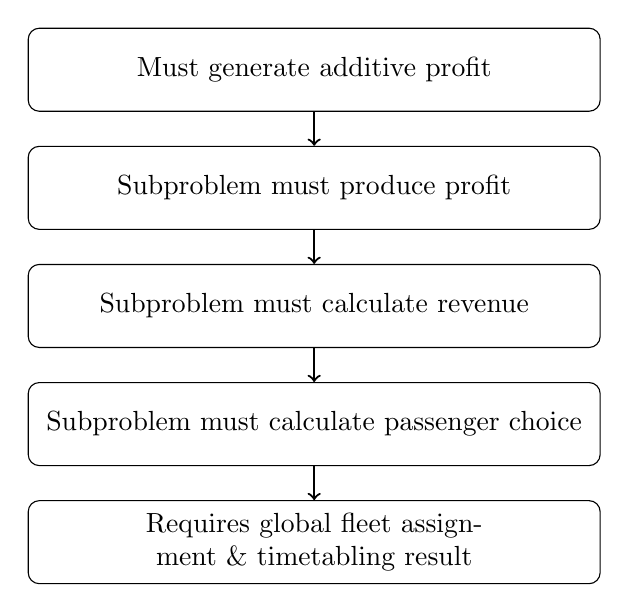
\begin{tikzpicture}[node distance=1.5cm, auto,
    block/.style={rectangle, draw, fill=white, text width=20em, text centered, rounded corners, minimum height=3em},
    line/.style={draw, ->, thick}]
    \node [block] (profit) {Must generate additive profit};
    \node [block, below of=profit] (sub_profit) {Subproblem must produce profit};
    \node [block, below of=sub_profit] (sub_rev) {Subproblem must calculate revenue};
    \node [block, below of=sub_rev] (sub_choice) {Subproblem must calculate passenger choice};
    \node [block, below of=sub_choice] (global) {Requires global fleet assignment \& timetabling result};

    \path [line] (profit) -- (sub_profit);
    \path [line] (sub_profit) -- (sub_rev);
    \path [line] (sub_rev) -- (sub_choice);
    \path [line] (sub_choice) -- (global);
\end{tikzpicture}
\caption{Logical dependency chain in Column Generation for ATFP}
\label{fig:cg_logic}
\end{figure}

This demonstrates that column generation is not a viable exact algorithm for ATFP.

\section{Mathematical and Methodological Argument}

The argument can be organized into a four-step incompatibility chain:

\subsection*{1. ATFP Objective Function is an Indivisible Profit Function}

The objective of ATFP is:
\[
\max \quad \text{Profit} = \text{Revenue}(\text{Schedule}, \text{Fleet}) - \text{Cost}(\text{Schedule}, \text{Fleet})
\]
where:
\begin{itemize}
    \item \textbf{Cost}: Determined by fleet assignment and timetabling. It is additive, arc-based, and schedule-based.
    \item \textbf{Revenue}: Derived from passenger choice. It is a global function.
\end{itemize}
This is a fact of the problem structure, not a modeling choice.

\subsection*{2. Passenger Choice is Globally Coupled}

In passenger choice models (whether Logit, Nested Logit, or SBLP), the attractiveness and selection probability of each itinerary depend on the \textbf{complete, global schedule and fleet assignment}.

Formally, the revenue is calculated as:
\[
\text{Revenue} = \sum_{m \in \marketSet} \sum_{p \in \psgTypeSet} \demand_{mp} \sum_{r \in \itinInMarket_m} \sum_{\ell \in \fareClassSet} \frac{\attr_{rp\ell}(\text{Schedule}, \text{Fleet})}{\outAttr_{mp} + \sum_{r' \in \itinInMarket_m} \sum_{\ell' \in \fareClassSet} \attr_{r'p\ell'}(\text{Schedule}, \text{Fleet})} \cdot \fare_{r\ell}
\]
Thus, \textbf{Revenue is not itinerary-level additive}, but rather a \textbf{solution-level functional}. This is the fundamental difference between ATFP and classical Crew Pairing or Fleet Assignment Models (FAM).

\subsection*{3. Necessary Condition for Column Generation: Additive Objective Function}

Standard Column Generation (CG) or Branch-and-Price requires:
\begin{itemize}
    \item Master problem:
    \[
    \max \sum_{r \in \itinSet} c_r \lambda_r
    \]
    \item Each column $r$:
    \begin{itemize}
        \item Has a \textbf{well-defined profit/cost independent of other columns}.
        \item Reduced cost can be corrected by dual variables.
    \end{itemize}
\end{itemize}
In other words, \textbf{each column generated by the subproblem must carry a "locally computable contribution value".}

\subsection*{4. This Condition is Violated by Passenger Choice in ATFP}

This is the fatal contradiction:
\begin{itemize}
    \item The subproblem must generate profit.
    \item Profit must include revenue.
    \item Revenue depends on passenger choice.
    \item Passenger choice depends on the global schedule and fleet assignment.
    \item However, in CG, when the subproblem generates a column, the global solution is not yet determined.
\end{itemize}

Therefore:
\begin{itemize}
    \item The subproblem \textbf{cannot define a correct revenue}.
    \item Consequently, it \textbf{cannot define a correct reduced cost}.
    \item Thus, the optimality criterion of CG fails, and "exact CG" is logically invalid.
\end{itemize}
This is not a difficulty in implementation, but an invalidity in definition.

\section{Conclusion on the Applicability of Column Generation}

While the above proves that standard column generation is incompatible with ATFP, for the sake of academic rigor, the statement should be refined:
\textbf{Standard column generation with profit-bearing columns is incompatible with ATFP under general passenger choice models.}

\subsection*{Restricted Cases where CG might apply}

CG might be applicable in extremely restricted cases where passenger choice is linearized or fixed, such as:
\begin{itemize}
    \item Fixed demand.
    \item Fixed revenue per flight.
    \item Choice calculated in a preprocessing stage.
\end{itemize}
In these cases, revenue degenerates to being arc-additive, and CG becomes applicable. However, this is \textbf{no longer ATFP} in its full sense.

\section{Summary}

Due to the presence of passenger choice, the revenue component in ATFP is inherently global and depends on the complete schedule and fleet assignment. As a result, individual decision components do not admit well-defined marginal profit contributions. This violates the additivity requirement underlying standard column generation and branch-and-price frameworks. Consequently, exact algorithms for ATFP cannot rely on profit-generating columns without resorting to strong approximations or restrictive assumptions on passenger behavior.
